\documentclass[twocolumn]{searchchev_preprint}
\usepackage{graphicx}
\newcommand{\nCconf}{82}
\newcommand{\nCconfhi}{83}
\newcommand{\nCconflo}{80}
\newcommand{\nChighamp}{96--98}
\newcommand{\nClongPhi}{62}
\newcommand{\nClongPlo}{46}
\newcommand{\nClowamp}{46--57}
\newcommand{\nCraw}{75}
\newcommand{\nCrawhi}{77}
\newcommand{\nCrawlo}{74}
\newcommand{\nCsc}{77}
\newcommand{\nCschi}{78}
\newcommand{\nCsclo}{75}
\newcommand{\nCshortP}{89--91}
\newcommand{\nFlongN}{1,262}
\newcommand{\nFlongRS}{829}
\newcommand{\nFlongSOL}{173}
\newcommand{\nFshortECL}{4,703}
\newcommand{\nFshortN}{6,268}
\newcommand{\nFshortRR}{565}
\newcommand{\nGdropConf}{6}
\newcommand{\nGdropRaw}{11}
\newcommand{\nMGmed}{8.1}
\newcommand{\nMconf}{18}
\newcommand{\nMraw}{25}
\newcommand{\nMsc}{23}
\newcommand{\nPknown}{1.3}
\newcommand{\nPmax}{351}
\newcommand{\nPmed}{1.4}
\newcommand{\nPmin}{0.035}
\newcommand{\nPminmain}{0.10}
\newcommand{\nPunk}{2.3}
\newcommand{\nampknown}{0.123}
\newcommand{\nampmed}{0.12}
\newcommand{\nampunk}{0.097}
\newcommand{\narea}{10,700}
\newcommand{\nauc}{0.954}
\newcommand{\nauclo}{0.939}
\newcommand{\naucshuf}{0.494}
\newcommand{\nbprpknown}{2.05}
\newcommand{\nbprpunk}{2.39}
\newcommand{\ndF}{9,130}
\newcommand{\ndFfrac}{15.6}
\newcommand{\ndQ}{2,980}
\newcommand{\ndQconf}{2,018}
\newcommand{\ndQext}{1,460}
\newcommand{\ndQgnb}{108}
\newcommand{\ndQvet}{558}
\newcommand{\ndfeat}{58,444}
\newcommand{\ndflag}{100,681}
\newcommand{\ndmatch}{92,249}
\newcommand{\ndrop}{2}
\newcommand{\ndtiles}{280}
\newcommand{\nextASASSN}{1,805}
\newcommand{\nextATLAS}{8,333}
\newcommand{\nextChen}{4,926}
\newcommand{\nextVSX}{6,369}
\newcommand{\ngradeC}{1,889}
\newcommand{\nhits}{31,089}
\newcommand{\nhitsknown}{17,027}
\newcommand{\nhitsknownext}{16,360}
\newcommand{\nhitsknowngaianb}{667}
\newcommand{\nhitsknownother}{0}
\newcommand{\nhitsmain}{30,703}
\newcommand{\nhitsshort}{386}
\newcommand{\nhitstovet}{14,062}
\newcommand{\nhitsunver}{837}
\newcommand{\nisodens}{3,770}
\newcommand{\nisofrac}{0.8}
\newcommand{\nknownany}{5,053}
\newcommand{\nmissedlo}{22,138}
\newcommand{\nnA}{3,210}
\newcommand{\nnAB}{5,778}
\newcommand{\nnABecl}{3}
\newcommand{\nnABshort}{38}
\newcommand{\nnB}{2,568}
\newcommand{\nnEcl}{166}
\newcommand{\nnLPV}{13}
\newcommand{\nnRR}{34}
\newcommand{\nnRS}{136}
\newcommand{\nncmd}{4,450}
\newcommand{\nncontrol}{550}
\newcommand{\nnew}{32}
\newcommand{\nnobsdiff}{-3}
\newcommand{\nnobsp}{0.33}
\newcommand{\nnocat}{90}
\newcommand{\nnotknownnoimg}{635}
\newcommand{\nnpairs}{391}
\newcommand{\nnseasonuntested}{108}
\newcommand{\nnvalneg}{4,000}
\newcommand{\nnvalpos}{356}
\newcommand{\npass}{7,667}
\newcommand{\nquiet}{40,386,274}
\newcommand{\nquietM}{40.4}
\newcommand{\nrecEcl}{77}
\newcommand{\nrecLPV}{8}
\newcommand{\nrecRR}{94}
\newcommand{\nrecRS}{46}
\newcommand{\nredfrac}{62}
\newcommand{\nrulefp}{9}
\newcommand{\nrulefpr}{0.22}
\newcommand{\nrulefprhi}{0.43}
\newcommand{\nrulerecall}{63}
\newcommand{\nruletp}{223}
\newcommand{\nscF}{8,879}
\newcommand{\nscFin}{8,913}
\newcommand{\nscFpct}{100}
\newcommand{\nscQ}{2,674}
\newcommand{\nscQin}{2,840}
\newcommand{\nscQpct}{94}
\newcommand{\nscopeabsent}{84}
\newcommand{\nscopeabsentpct}{1.5}
\newcommand{\nscopebelow}{676}
\newcommand{\nscopebelowpct}{11.7}
\newcommand{\nscopein}{5,760}
\newcommand{\nscopeknown}{5,000}
\newcommand{\nscopeknownpct}{86.8}
\newcommand{\nscopenofield}{18}
\newcommand{\nscored}{13,893,129}
\newcommand{\nscoredM}{13.9}
\newcommand{\ntiles}{2,796}
\newcommand{\nuncertain}{32}
\newcommand{\nvetpassfrac}{41}
\newcommand{\nweak}{24}

\begin{document}

\title{How many periodic variables did Gaia DR3 miss? A sealed-validation search of 13.9 million stars in ZTF,
with a pre-registered prediction for Gaia DR4}

\correspondingauthor{Deepnil Ray, \texttt{deepnilray\_ug2025@ashoka.edu.in}}
\author[0000-0001-8779-0700]{Deepnil Ray}
\affiliation{Ashoka University, Sonipat, Haryana 131029, India}
\affiliation{The NoRCEL Institute, United Kingdom}
\email{deepnilray\_ug2025@ashoka.edu.in}

\begin{abstract}
Gaia DR3 published variability results for about 10.5 million of its 1.8 billion sources. Every other star is
either constant or a variable that Gaia's pipeline did not flag, and the fraction of real variables it missed has
not been measured. I searched Zwicky Transient Facility (ZTF) DR23 light curves of \nscoredM\ million Gaia DR3 stars
with no variability result ($13\le G\le18.5$, \narea\ deg$^2$ at $|b|\ge15^\circ$) with a detector whose threshold was
fixed, and whose performance was measured, on sky tiles sealed before the search (AUC \nauc). Running the same
frozen detector on the stars Gaia \emph{did} flag, in a random 10\% of the searched sky, gives the fraction of
ZTF-detectable periodic variables that DR3 flagged: \nCraw--\nCconf\% overall (95\% ranges \nCrawlo--\nCconfhi\%),
and \nCsc\% when only variables confirmed by the independent ZTF SCoPe classifier are counted. The fraction falls from
about 90\% for periods below 0.5 d to \nClongPlo--\nClongPhi\% for periods of 1.6--160 d, and from \nChighamp\% at
amplitudes above 0.4 mag to \nClowamp\% at 0.05--0.1 mag; it depends only weakly on magnitude. Over the whole search
the detector found \nhitsmain\ periodic signals among Gaia-quiet stars; \nhitsknownext\ lie within $5''$ of an entry in a
published variable-star catalogue, and \nnAB\ others pass vetting that requires the period in at least two
independent light curves and across seasons. SCoPe lists \nscopeknownpct\% of those inside its coverage as variable.
Thirty-two are in no catalogue and pass image, contamination and light-curve checks; they are new, and include three
detached eclipsing binaries, one with a 25.4-d orbit. The catalogue and a prediction of what Gaia DR4 (2 December
2026) will report for these stars were deposited publicly before DR4.
\end{abstract}

\keywords{Variable stars (1761) --- Sky surveys (1464) --- Astronomy data analysis (1858) --- Eclipsing binary stars (444)}

\section{Introduction}
Gaia \citep{Gaia2016} DR3 \citep{Gaia2023} contains the largest homogeneous census of variable stars to date, built
by a pipeline that reports only the sources it identified as variable \citep{Eyer2023,Rimoldini2023}. A star absent
from the variability tables may be constant, or it may be a real variable that the pipeline missed because of Gaia's
sparse, scanning-law-driven sampling, a small amplitude, or its brightness. \citet{Everall2022} describe a selection
function for Gaia's variable samples as ``hugely valuable'' and note that building one requires knowing which sources
Gaia would have classified as variable had they been variable. To my knowledge, the fraction of real periodic
variables that DR3 left unflagged has not been measured as a function of period, amplitude and magnitude.

A ground-based survey with dense, multi-year sampling can measure it directly. ZTF \citep{Bellm2019,Masci2019} has
observed the northern sky every few nights since 2018. Large ZTF variable catalogues exist
\citep{Chen2020,Ofek2020,Healy2024}, and their question is how many variables ZTF contains. The question here is
narrower: of the periodic variables that one fixed ZTF detector finds, what fraction did Gaia DR3 flag, which kinds
did it miss, and how many such variables are there among the stars it called quiet.

Three design choices make the answer checkable. The detector and its threshold were frozen and validated on sealed
data before the search (\S\ref{sec:val}). The same frozen detector was run, unchanged, on Gaia-flagged and Gaia-quiet
stars in the same sky, so that the two counts share every selection effect of the ZTF side (\S\ref{sec:sf}). And the
rules that decide what is claimed, the frozen catalogue and a prediction for Gaia DR4 were made public before DR4
(\S\ref{sec:dr4}).

\section{Data}
\subsection{Targets}
I selected Gaia DR3 sources with $13\le G\le18.5$, RUWE $<1.4$, no entry in \texttt{vari\_summary} and
\texttt{phot\_variable\_flag} not equal to VARIABLE, at $|b|\ge15^\circ$ and $\delta\ge-25^\circ$. The sky was divided
into the HEALPix partitions of the ZTF HATS archive (orders 4, 5 and 6; 13.4, 3.36 and 0.84 deg$^2$). At the
catalogue freeze (27 November 2026, 03:45 UTC), \ntiles\ partitions (136, 2,646 and 14 of the three orders;
\narea\ deg$^2$) had been searched. They contain \nquietM\ million such stars. Of these, \nscoredM\ million have an
isolated, matched ZTF $r$-band light curve with at least 60 epochs and enough scatter to pass a pre-filter that keeps
95\% of the known variables in the sealed validation set (interquartile range over median error), and were scored by
the detector.

\subsection{Light curves}
ZTF DR23 PSF-photometry light curves were read from the IRSA HATS archive. Each Gaia star was matched to the ZTF object with
the most epochs among those within $1.5''$, and stars with another target star within $3''$ were
dropped. The detector runs on the star's $r$-band light curve. Vetting (\S\ref{sec:vet}) then uses every $g$, $r$ and $i$
light curve of the star (different fields, CCD quadrants and filters), kept separate so that each can confirm the
others independently.

\section{Method}
\subsection{Detector}
For each light curve I compute shape features: the Lomb--Scargle \citep{Lomb1976,Scargle1982} period over 0.1--200 d,
its power and false-alarm probability, the amplitude as the 5--95\% range of the magnitudes, amplitude over median
photometric error, reduced $\chi^2$ about the mean, skewness, the von Neumann ratio, and the output of a box-fit
eclipse channel for detached eclipsing binaries. A gradient-boosted decision-tree classifier maps the features to a
score. A light curve passes the periodic channel if $\log_{10}{\rm FAP}\le-6$, the amplitude is at least five times the
median error, and the period is not within 2\% of 0.5, 1 or 2 d, a lunar month or a year; the eclipse channel has its
own box-fit criteria. A star is a search hit if its score is above the frozen threshold, at least one channel passes,
and each half of the light curve, split in time, recovers the period independently (within 3\%, allowing factors 0.5
and 2; for the eclipse channel, both halves must also show a significant dip). For eclipsing binaries and other variables with two similar minima, the Lomb--Scargle period can be half the
true one.

A separate short-period channel covers 20 min to 2.4 h, below the detector's 0.1-d floor. It is run on stars with
reduced $\chi^2>2.5$ that are not already hits, and keeps a star when $\log_{10}{\rm FAP}<-10$, the semi-amplitude is
at least three times the median error, the frequency is not within 0.02 d$^{-1}$ of a whole number of cycles per day
or a harmonic of a longer significant period, and both halves of the light curve recover it. It contributed
\nhitsshort\ hits and \nnABshort\ catalogue stars, and is not used in the selection function.

\subsection{Sealed validation}\label{sec:val}
Before any light curve was downloaded, a seeded manifest assigned every tile to training, validation or search. The
classifier was trained on Gaia DR3 classified variables (positives) and Gaia-quiet stars (negatives) from training
tiles only, with positives restricted to classes ZTF can see (eclipsing, RR Lyrae, Cepheid, long-period, RS CVn, young
stellar and cataclysmic variables), and its threshold was set from out-of-fold scores on training data. Both were
then frozen, and only then were the validation tiles opened, once. On \nnvalpos\ Gaia-classified variables and
\nnvalneg\ Gaia-quiet stars in the validation tiles the classifier reached AUC \nauc\ (lower 95\% bound \nauclo),
against \naucshuf\ for a shuffled-label control. The score threshold together with a passing channel recovers
\nrulerecall\% of the sealed Gaia variables (\nrecEcl\% of \nnEcl\ eclipsing binaries, \nrecRR\% of \nnRR\ RR Lyrae,
\nrecRS\% of \nnRS\ RS CVn stars, \nrecLPV\% of \nnLPV\ long-period variables) and fires on \nrulefp\ of the
\nnvalneg\ quiet stars (\nrulefpr\%, upper 95\% bound \nrulefprhi\%). That rate is an upper limit on false positives,
because some of the ``negatives'' are unflagged variables of exactly the kind this search looks for; the season split,
applied in the search, further reduces it.

\subsection{Prior art at search time}
Every search hit was checked within $5''$ against 17 published variable-star catalogues through VizieR (VSX,
\citealt{Watson2006}; the ZTF catalogue of \citealt{Chen2020}, including its suspected variables, and a later ZTF
machine-learning catalogue; ASAS-SN; ATLAS; CRTS; WISE; TESS eclipsing-binary and period catalogues; and the Gaia
DR3 classification, rotation and eclipsing-binary tables, with their VizieR identifiers listed in the code) and a
published list of ZTF eclipsing white dwarfs. A hit with a match was marked known and was not vetted further. Because a Gaia-quiet star has, by construction, no
entry in the Gaia DR3 variability tables, a match there is a different source within $5''$; such hits are counted
separately below.

\subsection{Vetting rules}\label{sec:vet}
A hit not matched at search time becomes a catalogue star only if (i) its period is recovered in at least two
independent ZTF light curves; (ii) the period is detected in at least half (and at least two) of the observing seasons
tested; (iii) neither the period nor twice it lies within 1\% of a sampling alias (1/3, 1/2, 1 and 2 d, half and one
lunar month, half and one year); (iv) for periods above 1 d, the phases are evenly covered; and (v) no brighter Gaia
star lies within $6''$, and none two magnitudes brighter within $12''$. A star failing any of these, or sharing its
period with other stars in the same tile, is graded C and never claimed. The others are graded A (amplitude
$\ge0.08$ mag with at least three agreeing light curves in both $g$ and $r$, or amplitude $\ge0.15$ mag with two) or B.
Only grades A and B form the catalogue.

\subsection{Pre-registered decision rules}
The rules that decide what is claimed were committed publicly on 24 November 2026, before the catalogue was frozen
(see the repository history): when the catalogue freezes; that a catalogue star is known, and not claimed as new, if
it appears in VSX within $5''$ (or within $30''$ with the same period), in any of 17 VizieR variable-star catalogues,
in SIMBAD with a variable-star type, in ALeRCE \citep{SanchezSaez2021} with a periodic class at probability $\ge0.8$,
or in the latest SCoPe release \citep{Healy2024} with variable probability $\ge0.8$ and either a class probability
$\ge0.8$ or a matching period (factors 0.5, 1 or 2, within 1\%); and that every surviving star is inspected on sky
images. A check that fails is retried, and a star it still cannot check is not claimed. The selection-function
measurement of \S\ref{sec:sf} and its binning were registered in the same document.

\subsection{Contamination checks}
Every catalogue star that is listed as variable in no other catalogue was inspected on Pan-STARRS1 \citep{Chambers2016} $gri$
images ($40''$ cutouts). Galaxies and blends within $3''$ were dropped. Two further conditions move a star to
``uncertain'': a known variable within $30''$, whose light could leak into the ZTF photometry, or a ZTF magnitude more
than 0.5 mag brighter than Gaia $G$ with no Gaia $G_{BP}-G_{RP}$, a sign of a blend that Gaia resolves. Finally every
light curve was inspected by eye, and only those with a coherent shape well above the scatter in both bands are
claimed.

\subsection{Use of AI tools}
The analysis code was developed, and the analysis and drafting of this manuscript were carried out, with the
assistance of an AI system (Claude, Anthropic). The author designed and directed the work, checked every number
against the data files and code, and takes full responsibility for the content. Every number in the text is generated
by a script from the archived data (Data availability).

\section{What fraction of periodic variables did Gaia DR3 flag?}\label{sec:sf}
\subsection{Design}
In a random 10\% of the searched partitions (\ndtiles, drawn with a fixed seed and listed in the archive), I ran the
frozen detector, unchanged, on the Gaia DR3 stars that Gaia \emph{did} flag (an entry in \texttt{vari\_summary} or
\texttt{phot\_variable\_flag} = VARIABLE), with the same magnitude range, RUWE cut, cross-match, isolation criterion,
pre-filter, score threshold, channels and season split as the search. Of \ndflag\ flagged stars, \ndmatch\ have a ZTF
light curve and \ndfeat\ pass the pre-filter; the detector finds \ndF\ of them (\ndFfrac\%). In the same partitions the
search found \ndQ\ Gaia-quiet stars. Because the two groups pass through an identical ZTF selection, the fraction of
ZTF-detected periodic variables that DR3 flagged is
\begin{equation}
C = \frac{N_{\rm flagged}}{N_{\rm flagged}+N_{\rm quiet}},
\end{equation}
where both counts are detections by the frozen detector. $C$ measures DR3 against variables this ZTF detector can
find, so it says nothing about variables too faint, too low in amplitude or too long in period for ZTF.

\subsection{What counts as a real detection}
A detection among Gaia-quiet stars may be spurious, which would make $C$ too low. I therefore use three counts of
$N_{\rm quiet}$. The first counts every detection (\ndQ). The second counts only detections with independent support,
either a published catalogue entry within $5''$ (excluding the \ndQgnb\ whose only match is a neighbouring Gaia variable)
or a pass through the vetting of \S\ref{sec:vet}: \ndQconf\ stars (\ndQext\ catalogued and \ndQvet\ vetted). Counting
every vetting failure as spurious makes this a conservative choice. The third is symmetric: SCoPe classifies ZTF
light curves keyed by Gaia source identifier, so a SCoPe match is the same star. Of the detections inside SCoPe's
coverage, it lists \nscFpct\% of the Gaia-flagged ones (\nscF\ of \nscFin) and \nscQpct\% of the Gaia-quiet ones
(\nscQ\ of \nscQin) as variable at probability $\ge0.8$. Counting only SCoPe-confirmed variables on both sides removes
false detections from both groups in the same way.

\subsection{Result}
DR3 flagged \nCraw\% of the ZTF-detected periodic variables counting every detection and \nCconf\% counting supported
detections only (95\% ranges from a bootstrap over partitions: \nCrawlo--\nCrawhi\% and \nCconflo--\nCconfhi\%). With
SCoPe-confirmed variables on both sides the fraction is \nCsc\% (\nCsclo--\nCschi\%). Within this footprint and
magnitude range, therefore, roughly one ZTF-detectable periodic variable in five was left without a DR3 variability
result.

The missed fraction is far from uniform (Figure~\ref{fig:sf}, Table~\ref{tab:sf}). DR3 flagged about 90\% of
variables with periods below 0.5 d (where Gaia classifies \nFshortECL\ of the \nFshortN\ flagged detections as eclipsing
binaries and \nFshortRR\ as RR Lyrae stars), but only \nClongPlo--\nClongPhi\% of
those with periods between 1.6 and 160 d. It flagged \nChighamp\% of variables with amplitudes above 0.4 mag and
\nClowamp\% of those with amplitudes of 0.05--0.1 mag. Among the flagged detections at 1.6--160 d,
Gaia classifies \nFlongRS\ of \nFlongN\ as RS CVn and \nFlongSOL\ as solar-like variables, both classes of spotted stars.
The dependence on $G$ is weak: the flagged fraction is \nGdropConf--\nGdropRaw\ percentage points lower at $G=16$--18 than
at $G=13$--15. DR3 therefore missed mainly low-amplitude variability at multi-day periods, the regime of starspot
modulation on cool dwarfs, which is what most catalogue stars are (\S\ref{sec:pop}).

\begin{figure*}
\centering
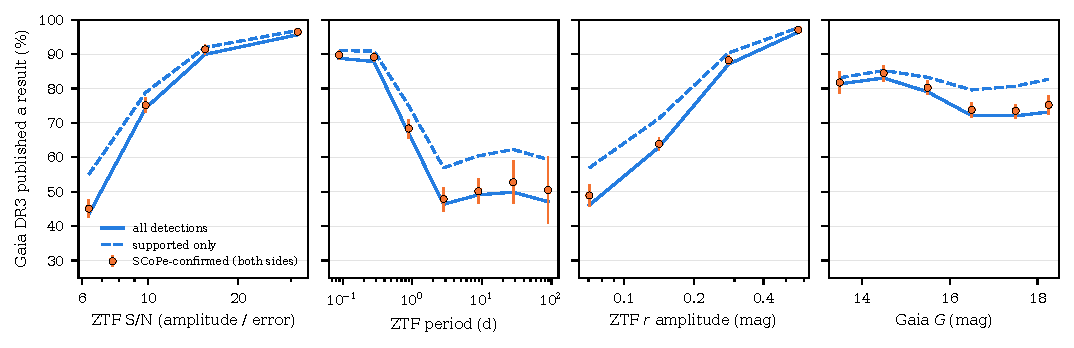
\includegraphics[width=0.98\textwidth]{fig_sf.pdf}
\caption{Fraction of ZTF-detected periodic variables that Gaia DR3 flagged, in the bins registered before the
measurement, against ZTF period, amplitude and $G$, in \ndtiles\ randomly chosen partitions. Solid line: every
detection counted; dashed line: Gaia-quiet detections counted only if catalogued within $5''$ or passing vetting; the
shaded band spans the 95\% Wilson intervals of the two. Points: SCoPe-confirmed variables only, on both sides. Bins
with fewer than 30 stars are omitted.\label{fig:sf}}
\end{figure*}

\input{sf_table.tex}

\section{The catalogue}
\subsection{From detections to catalogue}
Table~\ref{tab:res} follows every detection at the freeze. The detector found \nhits\ Gaia-quiet stars with a
confirmed periodic signal (\nhitsmain\ in the main channels and \nhitsshort\ in the short-period channel). Of these,
\nhitsknown\ were matched to a published catalogue at search time: \nhitsknownext\ to catalogues other than Gaia's own
(VSX \nextVSX, ATLAS \nextATLAS, \citealt{Chen2020} \nextChen, ASAS-SN \nextASASSN, with overlaps), \nhitsknowngaianb\
only to a Gaia DR3 variable within $5''$, and \nhitsknownother\ only to catalogues without periods or types. The
matched stars are reported in the archive but not claimed individually, because a $5''$ match does not prove that the
catalogued variable and the Gaia source are the same star. The remaining \nhitstovet\ hits were vetted, and \nnAB\
(\nnA\ grade A, \nnB\ grade B) form the catalogue analysed below. Their periods run from \nPmin\ d to \nPmax\ d (median
\nPmed\ d) and their median $r$-band amplitude is \nampmed\ mag (Figure~\ref{fig:pamp}).

\begin{deluxetable}{lc}
\tablecaption{From detections to catalogue, at the freeze (27 November 2026, 03:45 UTC).\label{tab:res}}
\tablehead{\colhead{Quantity} & \colhead{Value}}
\startdata
Partitions searched ($|b|\ge15^\circ$) & \ntiles\ (\narea\ deg$^2$) \\
Gaia-DR3-quiet stars, $13\le G\le18.5$ & \nquiet \\
\quad scored by the detector & \nscored \\
Confirmed periodic signals & \nhits \\
\quad matched to a published catalogue within $5''$ & \nhitsknown \\
\qquad to a non-Gaia catalogue & \nhitsknownext \\
\qquad only to a neighbouring Gaia DR3 variable & \nhitsknowngaianb \\
\quad vetted & \nhitstovet \\
\qquad passing vetting (A, B, C) & \npass \\
\qquad \textbf{catalogue (grade A or B)} & \textbf{\nnAB} \\
\quad in SCoPe as variable, matching class or period & \nscopeknown\ (\nscopeknownpct\%) \\
\quad in SCoPe below its variable threshold & \nscopebelow\ (\nscopebelowpct\%) \\
\quad absent from SCoPe & \nscopeabsent\ (\nscopeabsentpct\%) \\
\quad not in SCoPe's sky coverage & \nscopenofield \\
\quad known in any catalogue (pre-registered rules) & \nknownany \\
\quad in no catalogue & \nnocat \\
\qquad dropped (blend) & \ndrop \\
\qquad uncertain (possible blend or contamination) & \nuncertain \\
\qquad light curve too weak to claim & \nweak \\
\qquad \textbf{new variable stars} & \textbf{\nnew} \\
\enddata
\tablecomments{SCoPe percentages are of the \nscopein\ catalogue stars inside SCoPe's coverage. \nnotknownnoimg\ catalogue
stars are in SCoPe with a different class or period, or below its threshold, and are reported as independently
recovered, not as discoveries.}
\end{deluxetable}

\begin{figure*}
\centering
\includegraphics[width=0.82\textwidth]{fig_sky.pdf}
\caption{Sky positions (Galactic coordinates, Mollweide projection) of the \nnAB\ catalogue stars. Grey: already
classified as variable by another catalogue; blue: in no catalogue as a confirmed variable; orange stars: the \nnew\
new variables. The searched partitions lie at $|b|\ge15^\circ$ and $\delta\ge-25^\circ$.\label{fig:sky}}
\end{figure*}

\subsection{An external check: SCoPe}
SCoPe \citep{Healy2024} classified 1.65 billion ZTF light curves with its own features and models, independently of
this work. Of the \nscopein\ catalogue stars inside its coverage, it lists \nscopeknown\ (\nscopeknownpct\%) as variable
with a matching class or period. A detector that found noise or artefacts would not agree with an independent
classifier at this rate. A further \nscopebelow\ (\nscopebelowpct\%) are in SCoPe but below its own variable threshold,
or with a different period and class; for these the present work supplies a vetted period confirmed in independent
light curves and across seasons.

\subsection{New variable stars}
\nnocat\ catalogue stars are listed as variable in no catalogue. After the image, contamination and light-curve checks,
\nnew\ are claimed as new (Table~\ref{tab:new}, Figure~\ref{fig:lc}). They include three detached eclipsing binaries:
Gaia DR3 1198491283713804928 ($P=1.890$ d), 1052374297278903936 ($P=3.024$ d) and 346276760375634816, whose 25.4-d
orbit with narrow eclipses makes it a good target for radial-velocity follow-up. Two are contact binaries with periods
of 0.248 and 0.290 d. The others are periodic variables at 0.24 to 22 d with amplitudes of 0.06--0.32 mag; their types
are not assigned here, and for these the true period may be twice the ZTF period. A further \nweak\ stars passed every
catalogue and image check but have light curves too weak to claim; they are listed in the archive as candidates.

\begin{figure*}
\centering
\includegraphics[width=0.95\textwidth]{fig_lc.png}
\caption{Six of the new variables: ZTF $g$ (green, upper panels) and $r$ (red, lower panels) light curves folded at
the ZTF period (left of each pair) and twice it (right). From top left: the 25.4-d eclipsing binary
346276760375634816; the eclipsing binaries 1052374297278903936 and 1198491283713804928; the 22-d variable
321766687685841536; the 0.34-d variable 220985864201130880; and the 0.248-d contact binary 4230919197495489024.\label{fig:lc}}
\end{figure*}

\subsection{What kind of stars they are}\label{sec:pop}
Of the \nncmd\ catalogue stars with parallax over error above 5, \nredfrac\% have $G_{BP}-G_{RP}>1.8$ and the median
absolute magnitude is $M_G=\nMGmed$: almost all lie on the main sequence, and most are K and M dwarfs
(Figure~\ref{fig:cmd}). Among these, the stars no catalogue had classified are redder (median $G_{BP}-G_{RP}=\nbprpunk$
against \nbprpknown\ for the known ones). Across the whole catalogue they also have smaller amplitudes (median
\nampunk\ against \nampknown\ mag) and longer periods (median \nPunk\ against \nPknown\ d).

They were not under-sampled by Gaia. For \nnpairs\ catalogue stars paired with a quiet control star of matching
position, brightness and colour, the median paired difference in the number of Gaia DR3 $G$-band observations
(\texttt{phot\_g\_n\_obs}) is $\nnobsdiff$, and a Wilcoxon signed-rank test finds no difference ($p=\nnobsp$;
Figure~\ref{fig:nobs}). Together with \S\ref{sec:sf}, this points to small amplitude at multi-day periods, not the number
of Gaia observations, as the main reason these variables went unflagged.

\begin{figure}
\centering
\includegraphics[width=\columnwidth]{fig_pamp.pdf}
\caption{Period and amplitude of the \nnAB\ catalogue stars (colours as in Figure~\ref{fig:sky}).\label{fig:pamp}}
\end{figure}

\begin{figure}
\centering
\includegraphics[width=\columnwidth]{fig_cmd.pdf}
\caption{Gaia colour--absolute magnitude diagram of catalogue stars with parallax over error above 5 (colours as in
Figure~\ref{fig:sky}). Almost all are main-sequence stars, most of them K and M dwarfs.\label{fig:cmd}}
\end{figure}

\begin{figure}
\centering
\includegraphics[width=\columnwidth]{fig_nobs.pdf}
\caption{Number of Gaia DR3 $G$-band observations for \nnpairs\ catalogue stars and their matched quiet control stars.
The distributions are indistinguishable (Wilcoxon $p=\nnobsp$).\label{fig:nobs}}
\end{figure}

\section{Prediction for Gaia DR4}\label{sec:dr4}
The following was fixed, and deposited with its files, scoring script and SHA-256 hashes, on 27 November 2026, before
DR4 appears. Stars are matched through DR4's \texttt{dr3\_neighbourhood} table, with a $1''$ position match as a reported
fallback.

\textbf{P1.} DR4 flags a larger fraction of the \nnAB\ catalogue stars as VARIABLE than of \nncontrol\ control stars,
each chosen at random among Gaia-quiet stars within $0.5^\circ$ of a catalogue star with $|\Delta G|<0.25$ and
$|\Delta(G_{BP}-G_{RP})|<0.15$, at $z>3.3$. The POSSIBLE and NON\_VARIABLE fractions are reported separately.

\textbf{P2.} DR4 $G$-band light curves show the ZTF period (factor 0.5, 1 or 2, within 1\%) with false-alarm probability
$<10^{-3}$ more often for catalogue stars than for controls tested at their paired star's period.

\textbf{P3.} Among catalogue stars, the DR4 VARIABLE fraction rises with amplitude and falls for faint stars and for
periods beyond about 10 d, measured in bins fixed in advance (8 in $\log P$ over 0.05--500 d, 5 in amplitude, 1-mag bins
in $G$ from 12 to 19, Wilson intervals).

No target fraction is set, and the outcome will be reported whatever it is. DR4 also allows the measurement of
\S\ref{sec:sf} to be repeated with DR4 flags, giving the change in the flagged fraction between releases.

\section{Discussion}
The measurement of \S\ref{sec:sf} needs no model of Gaia's pipeline: it compares two groups of stars that a frozen
detector found in the same sky with the same light curves. The same design applies to any pair of surveys, and to
DR4 as soon as it is released. Its result is concrete. At $13\le G\le18.5$ and high latitude, DR3 flagged most short-period,
large-amplitude variables but only about half of the low-amplitude variables with periods of days to months, which in this
sample are mostly spotted K and M dwarfs. Studies that use the DR3 variability tables as a census of such stars, for
example of rotation or activity in the solar neighbourhood, should allow for this.

Two effects bias $C$ upward, so the missed fractions quoted here are more likely to be too small than too large.
The detector was trained with Gaia-classified variables as positives and Gaia-quiet stars, which include unflagged
variables, as negatives, so it may detect variables that resemble Gaia's flagged ones more efficiently than those
Gaia missed. And the $3''$ isolation test is applied within each group, so a Gaia-quiet star is dropped when another
quiet target lies within $3''$, while a flagged star is dropped only for another flagged star; at the mean target density
of the search (\nisodens\ deg$^{-2}$) about \nisofrac\% of stars have a target neighbour within $3''$, which bounds this
effect at under one percentage point in $C$.

Several further limitations should be stated plainly. $C$ is the flagged fraction among variables this detector finds, so
it does not include variables ZTF cannot detect, and it is measured only within $13\le G\le18.5$, RUWE $<1.4$, isolated
stars, $|b|\ge15^\circ$ and $\delta\ge-25^\circ$. The supported count of Gaia-quiet detections treats every vetting failure
as spurious and every $5''$ catalogue match as the same star; the SCoPe-only count avoids both assumptions but is
limited to SCoPe's coverage and threshold. Periods are Lomb--Scargle periods, so eclipsing and ellipsoidal binaries
appear at half their orbital period. The amplitude includes photometric noise and so overestimates the true amplitude
of the faintest stars. The ZTF DR1 candidates of \citet{Ofek2020} could not be obtained and were not checked against
the catalogue. Crowded low-latitude fields, where blending is worse, are not included.

The search continues on further partitions, and the DR4 test and a DR4 version of the selection function will follow
the release.

\section*{Data availability}
The frozen catalogue, the new-variable list, the DR4 prediction with its control list and scoring script, the image and
light-curve checks, and a code snapshot are archived on Zenodo (\href{https://doi.org/10.5281/zenodo.24579691}{doi:10.5281/zenodo.24579691},
published 27 November 2026). The selection-function inputs (search detections, detections among Gaia-flagged stars,
partition list and SCoPe lookups) and the script that generates every number in this paper are in the repository,
\url{https://github.com/deepnilray/SearchChev}.

\begin{acknowledgments}
I thank Prof. T. R. Seshadri (Ashoka University) for reviewing this project and for his advice on its method.
This work used data from the Zwicky Transient Facility, obtained through the NASA/IPAC Infrared Science Archive, and
data from the ESA mission Gaia, processed by the Gaia Data Processing and Analysis Consortium. It made use of the
ZTF SCoPe classifications, the ALeRCE broker, the AAVSO VSX catalogue, the SIMBAD and VizieR services of CDS, the
Pan-STARRS1 image archive, and the Gaia mirror of the Leibniz Institute for Astrophysics Potsdam. The use of AI tools
is described in the Method section.
\end{acknowledgments}

\section*{Conflicts of interest}
The author declares no conflicts of interest.

\begin{thebibliography}{}
\bibitem[Bellm et al.(2019)]{Bellm2019} Bellm, E. C., et al. 2019, PASP, 131, 018002
\bibitem[Chambers et al.(2016)]{Chambers2016} Chambers, K. C., et al. 2016, arXiv:1612.05560
\bibitem[Chen et al.(2020)]{Chen2020} Chen, X., et al. 2020, ApJS, 249, 18
\bibitem[Everall \& Boubert(2022)]{Everall2022} Everall, A., \& Boubert, D. 2022, MNRAS, 509, 6205
\bibitem[Eyer et al.(2023)]{Eyer2023} Eyer, L., et al. 2023, A\&A, 674, A13
\bibitem[Gaia Collaboration et al.(2016)]{Gaia2016} Gaia Collaboration, Prusti, T., et al. 2016, A\&A, 595, A1
\bibitem[Gaia Collaboration et al.(2023)]{Gaia2023} Gaia Collaboration, Vallenari, A., et al. 2023, A\&A, 674, A1
\bibitem[Healy et al.(2024)]{Healy2024} Healy, B. F., et al. 2024, ApJS, 272, 14
\bibitem[Lomb(1976)]{Lomb1976} Lomb, N. R. 1976, Ap\&SS, 39, 447
\bibitem[Masci et al.(2019)]{Masci2019} Masci, F. J., et al. 2019, PASP, 131, 018003
\bibitem[Ofek et al.(2020)]{Ofek2020} Ofek, E. O., et al. 2020, MNRAS, 499, 5782
\bibitem[Rimoldini et al.(2023)]{Rimoldini2023} Rimoldini, L., et al. 2023, A\&A, 674, A14
\bibitem[S\'anchez-S\'aez et al.(2021)]{SanchezSaez2021} S\'anchez-S\'aez, P., et al. 2021, AJ, 161, 141
\bibitem[Scargle(1982)]{Scargle1982} Scargle, J. D. 1982, ApJ, 263, 835
\bibitem[Watson et al.(2006)]{Watson2006} Watson, C. L., Henden, A. A., \& Price, A. 2006, SASS, 25, 47
\end{thebibliography}

\appendix
\section{The new variable stars}
\startlongtable
\begin{deluxetable*}{lrrrrrc}
\tablecaption{The \nnew\ new variable stars. $P$ is the orbital period for EA (detached eclipsing) and EW (contact)
binaries; for the others it is the ZTF period, and the true period may be twice it. Amp.\ is the ZTF $r$-band
5--95\% range.\label{tab:new}}
\tablehead{\colhead{Gaia DR3 source\_id} & \colhead{RA (deg)} & \colhead{Dec (deg)} & \colhead{$G$} & \colhead{$P$ (d)} & \colhead{Amp.} & \colhead{Type}}
\startdata
\input{table.tex}
\enddata
\end{deluxetable*}

\end{document}
